\documentclass{article}

\usepackage{graphicx}
\usepackage{hyperref}
\usepackage{tikz}
\usepackage{pgfplots}
\usepackage{siunitx}
\usepackage{float}


\author{Chirvasa Matei \& Rotariu George}
\title{Homework 0}

\begin{document}
\maketitle

\section{Introduction}
In this homework, we tackle the challenge of determining the global minimum of a multivariable function, on a small range, using a determinstic and a heuristic method.
\subsection{Motivation}
The motivation of this homework is to prove that certain computational problems are too resource-intensive to generate a correct response using a deterministic method, as well as show the consequences of using heuristic methods.

\section{Method}
\subsection{Functions}
For this demonstration we will use Rastrigin's Function\cite{Rastrigin}, Michalewicz's Function\cite{Michalwicz}, the Sum Square Function\cite{SumSquare}, and the Sphere Function\cite{Sphere}
\\Rastrigin's Function:
$$ f(x) = A \cdot n + \sum_{i=1}^n \left[ x_i^2 - A \cdot cos(2 \pi x_i) \right],
A = 10, x_i \in \left[ -1, 1 \right]$$

\begin{figure}[H]
  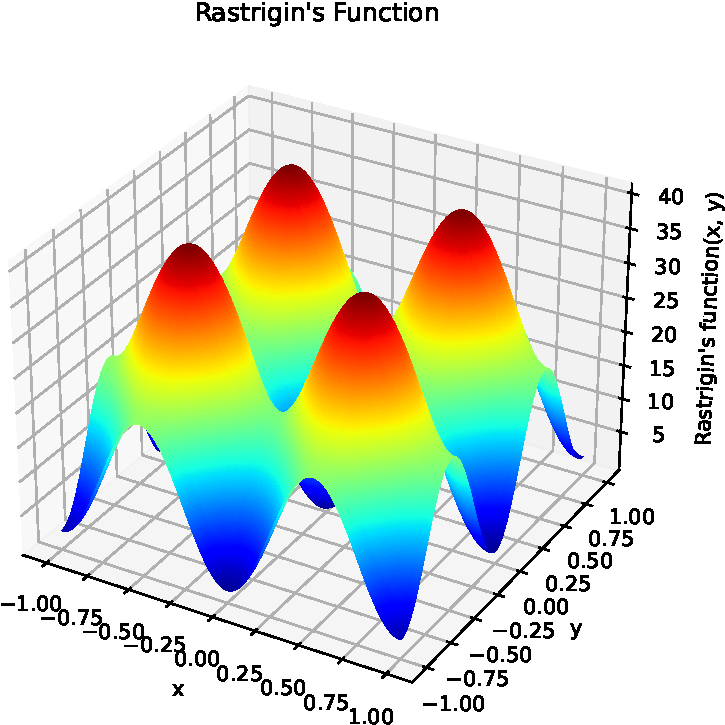
\includegraphics[]{Rastrigin_func-cropped}
  \caption{Rastrigin's Function.}
\end{figure}

Michalewicz's Function:
$$ f(x) = - \sum_{i=1}^n sin(x_i) \cdot sin^{2m}\left(\frac{i \cdot x_i^2}{\pi}\right),
m = 10, x_i \in \left[ 1, 3 \right]$$
\begin{figure}[H]
  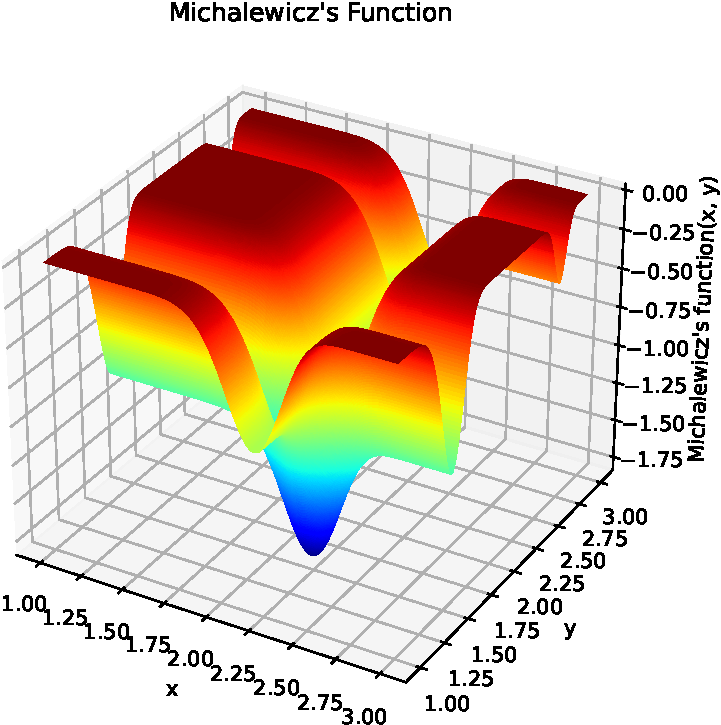
\includegraphics[]{Michalewicz_func-cropped}
  \caption{Michalewicz's Function}
\end{figure}

Shubert's Function:
$$ f(x) = \prod_{i = 1}^n i \cdot cos\left(\left(i + 1\right) \cdot x_i + i\right), x_i \in \left[ -1, 1 \right]$$
\begin{figure}[H]
  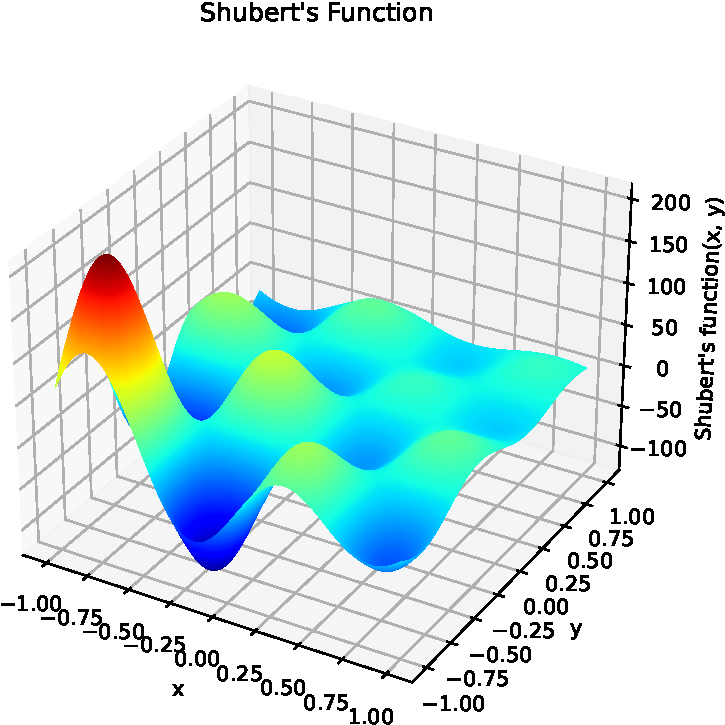
\includegraphics[]{Shubert_func-cropped}
  \caption{Shubert's Function}
\end{figure}

Sphere Function:
$$ f(x) = \sum_{i = 1}^n x_i^2, x_i \in \left[ -1, 1 \right]$$
\begin{figure}[H]
  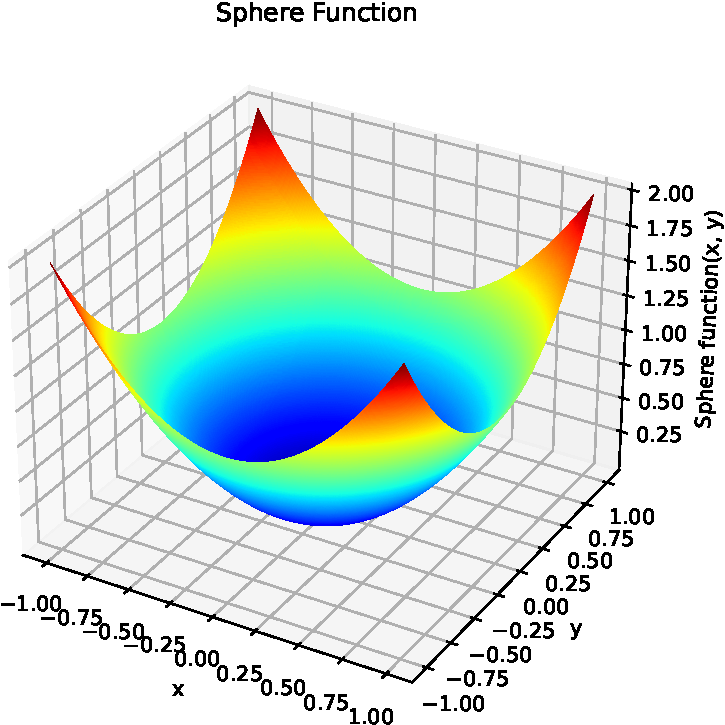
\includegraphics[]{Sphere_func-cropped}
  \caption{Sphere Function}
\end{figure}

\subsection{Algorithms}
For simplicity, algorithms will be ran with 2 and 10 dimensions.
\\For the determinstic method, we will use a simple algorithm that will generate every possible input $x = (x_1, x_2)$ or $(x_1, x_2, ..., x_9, x_{10})$, with a minimum $x_i$ step of $\varepsilon = \num{e-5}$ . Such an algorithm finds itself in the following complexity class:
$$O\left(\left(\frac{range}{\varepsilon}\right)^d\right), d = \text{Number of dimensions}$$
$$range = \text{Supremum} - \text{Infimum of the function's domain} $$

The algorithm will simply determine $f(x), \forall. x$ where $x_i$ $\in \left[ \text{infimum}, \text{supremum} \right]$.
\\As we know, exponential complexity algorithms are incredibly taxing on computers, and the estimated time required to run the algorithm multiple times may be too big for some time-sensitive tasks. Additionally, running this algorithm on 10-dimensional functions, with the specified $\varepsilon$ requires a number of steps that exceeds the upper limit of the bounds of the largest basic type in C++, that being size\_t. Thus, determining the correct answer for the function using a deterministic method is unfeasable.

The heuristic method will use an algorithm that will generate a random input $x$, and then search for the neighbour that yields the lowest result when the function is applied to it. If no neighbour gives a lower result than that of the current $x$, the algorithm stops, and assumes $x$ is the global minimum of the function. In truth, this algorithm produces a local minimum, chosen at random.
The complexity of such an algorithm is hard to estimate, as it depends on the amount of neighbours the current minimal point must pass through before finding a local minimum. However, we can estimate the amount of steps required to find the lowest neighbour of the current minimal point.
$$ O\left(3^d\right), d = \text{Number of dimensions} $$

This algorithm is also exponential, but given that $d \in \{2, 10\}$, compared to the determinstic method, the time required to run the function is meaningfully smaller.

\section{Experiment}

We will use C++ to implement the described algorithms, and we will run them in parallel using the std::async method of the $\langle\text{future}\rangle$ module. The heuristic methods on 2-dimensional functions are much quicker to execute, and will be ran on the main thread, while awaiting the execution of the asynchronous threads. The computer was also used for other daily activites, and such the duration results of the same function may significantly variate. 

\section{Results}

\begin{figure}[H]
\begin{tabular}{|c||c|c|c|c|}
  \hline
  Function Name & Global Minimum & Avg. Runtime(ms) & Min. Runtime(ms) & Max. Runtime(ms) \\ \hline \hline
  Rastrigin & 0 & 1287322.1 & 1036618 & 2264272 \\ \hline
  Michalewicz & -1.8013 & 1476872.5 & 1024324 & 2829847 \\ \hline
  Shubert & -123.57677 & 2807958.8 & 2297443 & 3369678 \\ \hline
  Sphere & 0 & 728667.4 & 478353 & 1257387 \\ \hline
\end{tabular}
\caption{Determinstic function run stats, over $\approx$ 10 runs}
\end{figure}

\begin{figure}[H]
\begin{tabular}{|c||c|c|}
  \hline
  Function Name & Success rate & Avg. Runtime(ms) \\ \hline \hline
  Rastrigin & 0.422594142 & 3.922222222 \\ \hline
  Michalewicz & 0.68 & 44.6 \\ \hline
  Shubert & 0.338888889 & 11.68333333 \\ \hline
  Sphere & 1 & 3.735294118 \\ \hline
\end{tabular}
\caption{Heuristic function run stats on 2-dimensional functions}
\end{figure}

\begin{figure}[H]
\begin{tabular}{|c||c|c|c|c|}
  \hline
  Function Name & Lowest Minimum & Avg. Runtime(ms) & Min. Runtime(ms) & Max. Runtime(ms) \\ \hline \hline
  Rastrigin & 0.99496 & 174612.4833 & 95671 & 364268 \\ \hline
  Michalewicz & -8.97945 & 1081169.957 & 341559 & 2331731 \\ \hline
  Shubert & -5585808058 & 453170.4333 & 215750 & 990436 \\ \hline
  Sphere & 0 & 169273.625 & 91360 & 340066 \\ \hline
\end{tabular}
\caption{Heuristic function run stats on 10-dimensional functions}
\end{figure}

\href{./h0data.xlsx}{Spreadsheet containing all function data}

\subsection{Interpretation}

\section{Conclusions}



\begin{thebibliography}{9}

\bibitem{Rastrigin}
  Wikipedia Commons \\ Rastrigin's Function rendered image.
  \url{https://en.wikipedia.org/wiki/Rastrigin_function}

\bibitem{Something}
  Rastrigin, L. A. "Systems of extremal control." Mir, Moscow (1974).
\end{thebibliography}  
\end{document}

